\def\year{2019}\relax
%File: formatting-instruction.tex
\documentclass[letterpaper]{article} %DO NOT CHANGE THIS
\usepackage{aaai19}  %Required
\usepackage{times}  %Required
\usepackage{helvet}  %Required
\usepackage{courier}  %Required
\usepackage{url}  %Required
\usepackage{graphicx}  %Required
\usepackage{subcaption}
\frenchspacing  %Required
\setlength{\pdfpagewidth}{8.5in}  %Required
\setlength{\pdfpageheight}{11in}  %Required
%PDF Info Is Required:
  \pdfinfo{
/Title(Tracking images of people in hotel rooms)
/Author(Abby Stylianou, Richard Souvenir, Jon Brandt (?), and Robert Pless)}
\setcounter{secnumdepth}{0} 
 \begin{document}
% The file aaai.sty is the style file for AAAI Press 
% proceedings, working notes, and technical reports.
%
\title{Tracking images of people in hotel rooms}
\author{Abby Stylianou, Richard Souvenir, Jon Brandt (?), and Robert Pless}
\maketitle
\begin{abstract}
We present a novel dataset of annotated hotel room images to support developing the state of the art in the challenging task of hotel recognition. Hotel recognition is both an interesting scene recognition challenge, as well as an important component in investigations of human trafficking. Photographs of victims in hotel rooms are often part of investigations of human trafficking -- law enforcement seek to identify where a victim was trafficked and where their trafficker might move them or others in the future. Identifying hotel rooms from photographs of victims is a surprisingly difficult scene recognition task due to both the properties of the victim photos, as well as the properties of hotel rooms. The victim photos are often of low quality, with large occlusions and varying perspectives. Hotel rooms are a challenging class of scene to recognize, for several reasons: rooms within the same hotel may have the same objects in very different configurations; they may have entirely different objects in different rooms as floors get renovated one at a time; and different hotels, especially those from the same chain, may have very similar objects. In this paper, we explore the implications of these challenges on deep learning based image retrieval systems, present a baseline approach to image retrieval that addresses some of these concerns, and release to the community a massive dataset of annotated hotel room images with the goal of improving the state of the art in hotel specific scene recognition to support investigations of human trafficking.
\end{abstract}

\begin{verbatim}
Key points:

1. Really important problem domain 
(have lots of text for this.)

2. Really interesting scene matching 
problem.

3. Large dataset + evaluation baseline 
w/ code available.
- Only hotels that have some # of TC and 
Expedia images
- 

4. No occlusion version, occluded version
and the object version create a 
progressively harder challenge, 
AND each of these problems.

Heirarchy of problems:
1. Whole room matching w/ TC queries
1A. Exact hotel
1B. Hotel chain
2. Occluded matching w/ TC queries 
pre-messed up with COCO occlusions.
3. Object specific search --- we create, as 
part of the test set, a query set of objects
in hotel rooms. Evaluation is given a query
of just an object, do you get the correct 
hotel?
\end{verbatim}
\noindent Text starts here.~\cite{netdissect2017}

\begin{figure*}
    \centering
    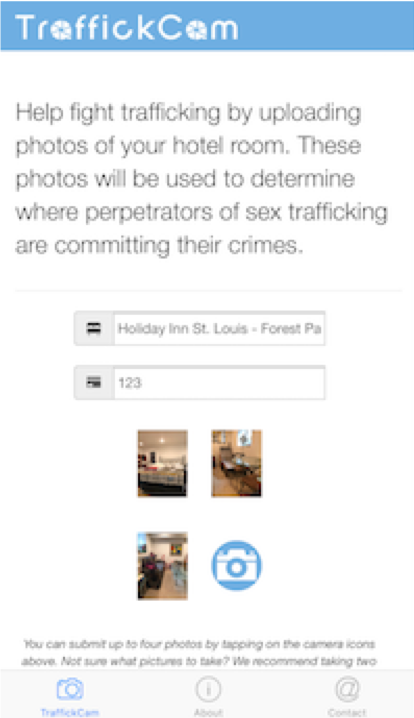
\includegraphics[height=2.4in]{figures/screenshots/1.png}
    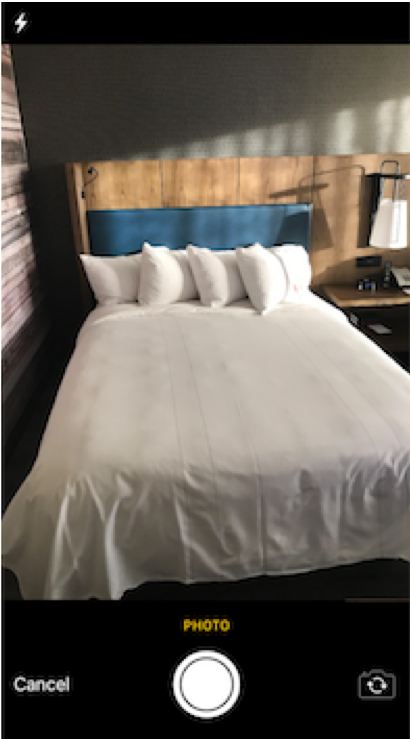
\includegraphics[height=2.4in]{figures/screenshots/2.png}
    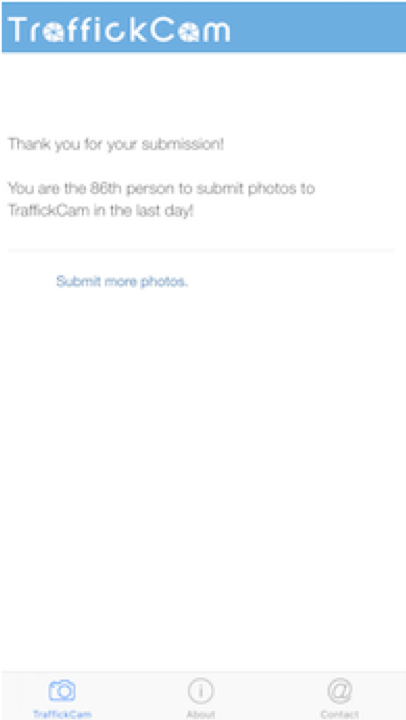
\includegraphics[height=2.4in]{figures/screenshots/3.png}
    \caption{Screenshots of the TraffickCam iOS application}
    \label{fig:tcamScreenshots}
\end{figure*}

\begin{figure*}
\centering
    \begin{subfigure}[b]{\textwidth}
    \centering
    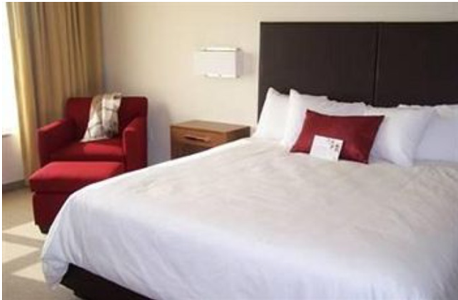
\includegraphics[height=1in]{figures/example_images/expedia/1.png}
    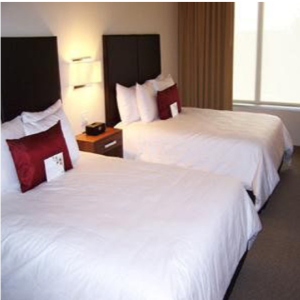
\includegraphics[height=1in]{figures/example_images/expedia/2.png}
    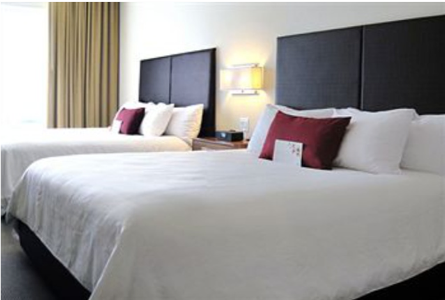
\includegraphics[height=1in]{figures/example_images/expedia/3.png}
    \caption{Web images}
    \end{subfigure}
    \\
   \begin{subfigure}[b]{.6\textwidth}
   \centering
    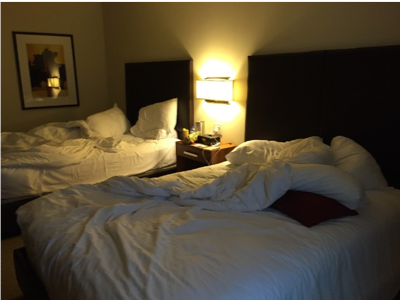
\includegraphics[height=1in]{figures/example_images/tcam/1.png}
    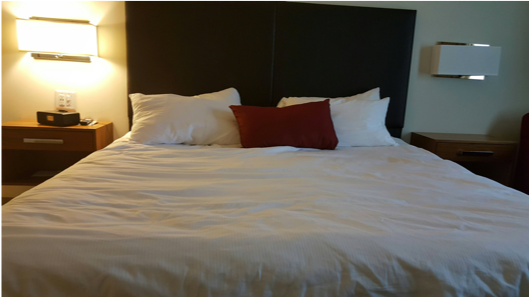
\includegraphics[height=1in]{figures/example_images/tcam/2.png}
    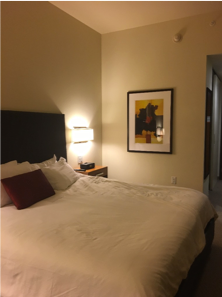
\includegraphics[height=1in]{figures/example_images/tcam/3.png}
    \caption{App images}
    \end{subfigure}
   \begin{subfigure}[b]{.3\textwidth}
   \centering
    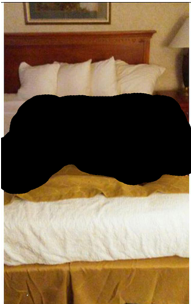
\includegraphics[height=1in]{figures/example_images/queries/1.png}
    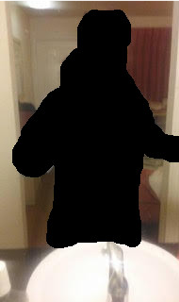
\includegraphics[height=1in]{figures/example_images/queries/2.png}
    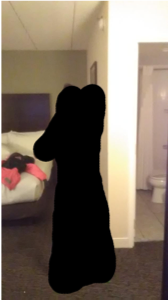
\includegraphics[height=1in]{figures/example_images/queries/3.png}
    \caption{Query images}
    \end{subfigure}
    \caption[Image variability from different sources]{Example images from (a) hotel websites, (b) the TraffickCam crowdsourcing app, and (c) queries used by law enforcement. The images in (a) and (b) are from the same hotel, highlighting the significant differences in the properties of images from different sources.}
    \label{fig:domainImages}
\end{figure*}

\section{Dataset}

If we only consider hotels that have both TraffickCam and Expedia images:
\begin{itemize}
\item 19,948 hotels from 97 chains
\item 182,200 TraffickCam images from 47,049 users
\item 370,591 Expedia images
\end{itemize}

Some questions/comments that we need to consider as we create this dataset:
\begin{itemize}
\item Should the query images in the test set consist of only TraffickCam images, emphasizing the domain transfer aspect of this problem?
\item When we evaluate a TraffickCam query image, we want to make sure there are no other images from that user in the test set.
\item Do we want to remove ALL other TraffickCam images from that hotel from the test set? Or, do we want to REQUIRE that there be TraffickCam images from another user at that hotel?
\item Should we include hotels that only have expedia images in the dataset?
What should the size/division of the training/validation/test sets be?
\end{itemize}


%References and End of Paper
%These lines must be placed at the end of your paper
\bibliography{bib}
\bibliographystyle{aaai}
\end{document}
